% Drawing 144/08-3 -- folder 144, batch 08, archive page 155 (PDF page 156).
% Transcription: en haut, deux figures d'un tore (ou d'une sphère à anse) traversé par un cylindre horizontal. Sur la première sont portées les étiquettes $X'$ (deux fois), $\xi'$, $X_0^{*}$ et, sur le cylindre, $\xi''$ et une flèche marquée $5$ \uncertain{ou} $S$ ; la seconde montre le même cylindre traversant une figure ovale, vue de face.
% Kind: ring (torus) pierced by a horizontal cylinder, two views. Method 2 (schematic redraw from the facsimile). Status: ok.
% Notes: First figure: the ring (doubled outline) pierced by a horizontal cylinder, with X' (twice), xi' (arrow), X_0^* and, on the cylinder, xi'' and an arrow marked 5 or S (as in the transcription). Second figure: the same cylinder through an oval seen from the front (its left end dashed).
% Coordinates: 1 unit = 1 mm = 1/100 of the crop width (bbox in page fractions: [0.15, 0.06, 0.58, 0.27]).
% Redrawn by Claude (claude-opus-5-5), issue #73, 2026-11-07; not checked by a human; not compiled (no TeX in the session).
% Rights: reproduces part of the work -- behind RENDER_TRANSCRIPTS, never published by itself.
\documentclass[tikz,border=3pt]{standalone}
\usepackage{amsmath,amssymb}
\usetikzlibrary{patterns,arrows.meta}
\tikzset{pencil/.style={black!45}, struck/.style={black!35}, mark/.style={circle,draw,inner sep=1.3pt}, pt/.style={circle,fill,inner sep=0.9pt}, opt/.style={circle,draw,fill=white,inner sep=1.1pt}}
\begin{document}
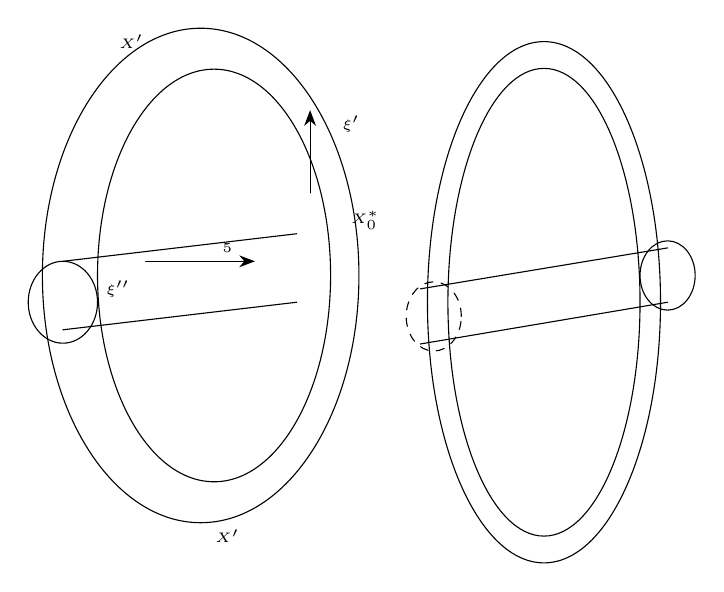
\begin{tikzpicture}[x=1mm,y=1mm,line cap=round,line join=round,font=\scriptsize]
\draw (32.6,-42.3) ellipse[x radius=20.1, y radius=31.4];
\draw (34.3,-42.3) ellipse[x radius=14.8, y radius=26.2];
\draw (15.1,-40.5) -- (44.8,-37);
\draw (15.1,-49.2) -- (44.8,-45.7);
\draw (15.1,-45.7) ellipse[x radius=4.4, y radius=5.2];
\draw[-{Stealth[length=2mm]}] (25.6,-40.5) -- (39.5,-40.5);
\draw[-{Stealth[length=2mm]}] (46.5,-31.8) -- (46.5,-21.3);
\node[inner sep=1pt] at (23.8,-12.6) {\tiny $X'$};
\node[inner sep=1pt] at (51.7,-23.1) {\tiny $\xi'$};
\node[inner sep=1pt] at (53.5,-35.3) {\tiny $X_0^*$};
\node[inner sep=1pt] at (36,-75.4) {\tiny $X'$};
\node[inner sep=1pt] at (22.1,-44) {\tiny $\xi''$};
\node[inner sep=1pt] at (36,-38.8) {\tiny $5$};
\draw (76.2,-45.7) ellipse[x radius=14.8, y radius=33.1];
\draw (76.2,-45.7) ellipse[x radius=12.2, y radius=29.7];
\draw (60.5,-44) -- (91.9,-38.8);
\draw (60.5,-51) -- (91.9,-45.7);
\draw (91.9,-42.3) ellipse[x radius=3.5, y radius=4.4];
\draw[dashed] (62.2,-47.5) ellipse[x radius=3.5, y radius=4.4];
\end{tikzpicture}
\end{document}
